\documentclass[twoside]{article}
\usepackage[utf8]{inputenc}
\usepackage{listings}
\usepackage[dvipsnames]{xcolor}


% The package supports other formats as well, but this template
% is primarily checked and updated for examinations at TUM BGDM

% with/without answers
% \usepackage[uebung, answers]{tumbgdm}
\usepackage[uebung]{tumbgdm}
% \setlength{\parskip}{\baselineskip}%
% \setlength{\parindent}{0pt}%
% \usepackage{pythonhighlight}
\usepackage[skip=6pt, indent=0pt]{parskip}
\usepackage{xcolor}
\hypersetup{
    colorlinks,
    linkcolor={red!50!black},
    citecolor={blue!50!black}, 
    urlcolor={blue!80!black}
}

\Professor{Prof. Dr. Martin Werner}
\Universitaet{Technical University of Munich}
\Institut{School of Engineering and Design}
\Lehrstuhl{Professorship Big Geospatial Data Management}
\Semester[WiSe XX/XX]{WiSe XX/XX}
\Vorlesung{Principles of Programming}
\InstitutsWebsite{https://www.bgd.ed.tum.de/}

\nummerUebungsblatt{1-40}
\nummerErsteFrage{1}


\LearningOutcome{Basic Computing}


\begin{document}
\maketitle


\newpage
\section{Python Environment}

\begin{task}{Environments and Jupyter Notebooks}{}{}

Create an environment and start a Jupyter Notebook:

\begin{lstlisting}[numbers=none]
python -m venv /path/to/my/envirnoment
source /path/to/my/envirnoment/bin/activate
pip install notebook
jupyter notebook
\end{lstlisting}

You can exit the environment by typing \textit{deactivate} in your shell.
If you want to use Anaconda, you may do this inside the "Anaconda Navigator" or execute the following lines:

\begin{lstlisting}[numbers=none]
conda create --name myfirstenv
conda activate myfirstenv
conda install notebook
jupyter notebook
\end{lstlisting}

You can exit the conda environment by typing \textit{conda deactivate} in your shell.

\end{task}

%Basic: https://pynative.com/python-basic-exercise-for-beginners/
\newpage
\begin{task}{Basic Python Exercise}{}{}
Solve the following tasks inside a Jupyter Notebook. An example follows each task.
\begin{enumerate}
    \item print "Hello, World"
    \begin{lstlisting}[numbers=none]
    Output: Hello, World
    \end{lstlisting}
    
    \item multiplicate two numbers
    \begin{lstlisting}[numbers=none]
    Input: 53, 834
    Output: 44679
    \end{lstlisting}
    
    \item remove first n characters from a string
    \begin{lstlisting}[numbers=none]
    Input: "Hello", 2
    Output: llo
    \end{lstlisting}

    \item check if the first and last number of a list are the same
    \begin{lstlisting}[numbers=none]
    Input: [5, 3, 1, 3, 4, 5]
    Output: True
    \end{lstlisting}
    
    
    \item return the count of a given substring from a given string
    \begin{lstlisting}[numbers=none]
    Input: "I have no idea what I am doing.", "I"
    Output: 2
    \end{lstlisting}
    
    \item check if a given number is a palindrome number
    \begin{lstlisting}[numbers=none]
    Input: 32123
    Output: True
    \end{lstlisting}
    
\end{enumerate}
\end{task}

\newpage
\begin{task}{Python Scripts}{}{}

    Install a code editor (e.g., VS Code) and create a Python script (e.g., tutorial\_1.py). Implement Task 2 a. - f. with a main function and run it.
    The basic structure of your script may look like the following:
    
    \begin{lstlisting}[numbers=none]
        def main():
            # Your code here ...           
            return result

        if __name__=="__main__":
            main()
    \end{lstlisting}

\end{task}


\begin{task}{Command Line Python}{}{}

    Run your Python script from Task 3 in the command prompt (Windows) or terminal (Linux) by typing \textit{python /path/to/tutorial\_1.py}.
    Then, do Task 2 a. - b. without a script by running Python directly in the shell.
    You can start Python from the command line by typing \textit{python}.

\end{task}


\newpage
\section{Python Loops}
\begin{task}{For Loops}{}{}
Use a for loop to print a multiplication table from 1 to 10.

\vspace{10pt}
Expected output:
\begin{lstlisting}[numbers=none]
1   2  3  4  5  6  7  8  9  10 		
2   4  6  8 10 12 14 16 18  20 		
3   6  9 12 15 18 21 24 27  30 		
4   8 12 16 20 24 28 32 36  40 		
5  10 15 20 25 30 35 40 45  50 		
6  12 18 24 30 36 42 48 54  60 		
7  14 21 28 35 42 49 56 63  70 		
8  16 24 32 40 48 56 64 72  80 		
9  18 27 36 45 54 63 72 81  90 		
10 20 30 40 50 60 70 80 90 100 
\end{lstlisting}

\end{task}

\begin{task}{While Loops}{}{}
Using a while statement, write a function that takes two int values ("base" and "exponent") as input and prints the base to the power of the exponent.

\vspace{10pt}
\textbf{Example}\\
Expected output for input base=2 and exp=5:
\begin{lstlisting}[numbers=none]
2 to the power of 5 is:  32
\end{lstlisting}

\end{task}


\clearpage
\newpage
\section{Python List Comprehensions}

Solve the following tasks with list comprehensions:
\begin{lstlisting}[numbers=none]
newlist = [expression for item in iterable if condition] 
\end{lstlisting}


\begin{task}{Reverse String}{}{}
Write a function that reverses a string.

\vspace{10pt}
\textbf{Example}\\
Expected output for input s = "hello":
\begin{lstlisting}[numbers=none]
["o","l","l","e","h"]
\end{lstlisting}

%\vspace{5pt}
%\textbf{Constraints:}
%\begin{itemize}
%    \item $1 \leq len(s) \leq 10^5$
%    \item s[i] is a printable ascii character.
%\end{itemize}
\end{task}


\begin{task}{Sort Array}{}{}
Given an integer array nums, move all the even integers at the beginning of the array followed by all the odd integers.
Return any array that satisfies this condition.

\vspace{10pt}
\textbf{Example}\\
Expected output for input nums = [3,1,2,4]:
\begin{lstlisting}[numbers=none]
[2,4,3,1]
\end{lstlisting}
Explanation: The outputs [4,2,3,1], [2,4,1,3], and [4,2,1,3] would also be accepted.

%\textbf{Constraints:}
%\begin{itemize}
%    \item $1 \leq len(nums) \leq 5000$
%    \item $0 \leq nums[i] \leq 5000$
%\end{itemize}
\end{task}

\newpage
\begin{task}{Fizz Buzz}{}{}
Fizz buzz is a group word game for children to teach them about division. Players take turns to count incrementally, replacing any number divisible by three with the word "fizz", and any number divisible by five with the word "buzz", and any number divisible by both 3 and 5 with the word "fizzbuzz" (from \href{https://en.wikipedia.org/wiki/Fizz_buzz}{Wikipedia}).\\

Given an integer n, return a string array answer (1-indexed) where:

\begin{enumerate}
    \item answer[i] == “FizzBuzz” if i is divisible by 3 and 5.
    \item answer[i] == “Fizz” if i is divisible by 3.
    \item answer[i] == “Buzz” if i is divisible by 5.
    \item answer[i] == i (as a string) if none of the above conditions are true.
\end{enumerate}

\vspace{10pt}
\textbf{Example}\\
Expected output for input n = 15:
\begin{lstlisting}[numbers=none]
["1","2","Fizz","4","Buzz","Fizz","7","8","Fizz","Buzz","11","Fizz","13","14","FizzBuzz"]
\end{lstlisting}

%\vspace{5pt}
%\textbf{Constraints:}
%\begin{itemize}
%    \item $1 \leq n \leq 10^4$
%\end{itemize}
\end{task}

\newpage
\begin{task}{Numpy}{}{}
%\begin{lstlisting}[numbers=none]
%import numpy as np
%\end{lstlisting}
Import the NumPy package (Official documentation: \href{https://numpy.org/doc/}{https://numpy.org/doc/}) and use it to solve the following tasks:

\begin{enumerate}
    \item Print the Numpy version and configuration
    \item Create a 10x10 matrix filled with zeros
    \item Find the shape of an arbitrary array (e.g. the one from a.)
    \item Create a 4x6 matrix with zeros but the value at index [2, 3] which is 1
    \item Create a 3x7 matrix filled with values ranging from 21 to 42
    \item Create a vector of size 10 filled with random values from 0 to 1
    \item Reverse the vector from f. (first element becomes last)
    \item Create a 3x3 matrix with random integer values ranging from 0 to 8
    \item Find indices of non-zero elements from [1,0,7,0,1,0,0,1,0,0,1]
    \item Find all unique values from [1,0,7,0,1,0,0,1,0,0,1]
    \item Create a 3x3 identity matrix
    \item Multiply a 5x3 matrix by a 3x2 matrix
    \item Create a random vector of size 10 and sort it
    \item Create a 5x5x5 array with random values and find the minimum, the maximum and the mean value
\end{enumerate}
\end{task}


\clearpage
\section{Matplotlib}
\begin{task}{Matplotlib}{}{}
%\begin{lstlisting}[numbers=none]
%from matplotlib import pyplot as plt
%\end{lstlisting}
Import the Pyplot package from Matplotlib (Official documentation: \href{https://matplotlib.org/stable/api/index.html}{https://matplotlib.org/stable/api/index.html}) and use it to solve the following tasks:

\begin{enumerate}
    \item Load an image of your choice
    \item Display the image
    \item What are the spatial dimensions, data type, and range of the values of the image?
    \item What is the color value of the pixel at position [21,42]?
    \item Calculate the mean colour value for each channel over all pixels
    \item Convert the image in grayscale and display it. The gray value h can be calculated from the RGB values using the formular h = 0.2989r + 0.5870g + 0.1140b.
    \item Change the colormap so that the image is actually shown as grayscale and display it again
    \item Save the grayscale image in the PNG-format
    \item Create and plot a histogram of the grayscale image
\end{enumerate}
\end{task}

\begin{task}{Numpy continued}{}{}
Use Numpy to solve the following tasks.
\begin{enumerate}
    \item Create a 2D array with 1 on the border and 0 inside
    \item Normalize a 5x5 random matrix
    \item Multiply a 4x3 matrix by a 3x5 matrix
    \item Create a random vector of size 6 and replace the maximum value by 0
    \item Create a 2D integer matrix and return the transpose
    \item Create a checkerboard 10x10 matrix using the "tile" function
\end{enumerate}
\end{task}



\newpage
\begin{task}{Matplotlib continued}{}{}
Use Matplotlib to solve the following tasks.
First, we create some random dataframe with pandas:
\begin{lstlisting}[numbers=none]
import pandas
df = pandas.DataFrame(data={"a":np.random.randint(0, 100, 50),
                            "b":np.random.randint(0, 100, 50),
                            "c":np.random.randint(0, 100, 50)})
\end{lstlisting}


\begin{enumerate}
    \item Create a figure of size 15x8 with two subplots, top and bottom
    \item Draw two lines (data a and b) in the top plot, one blue and one orange, and add a grid
    \item Create two vectors of size 50 filled with random values in range 0-10 and use "matplotlib.pyplot.fill\_between" function to plot an artificial standard deviation for both lines (Hint: Set "alpha=0.2" and "edgecolor=None")
    \item For the top plot, add a title and a legend in the top-middle
    \item In the bottom plot, create a graph of only the data points (c), marked by circles, but with no line connecting the points. Further, add a grid, title, and legend for the bottom plot
\end{enumerate}

\begin{enumerate}
    \item Create a figure of size (15,18) with three subplots, aligned vertically
    \item Create bar graphs for data a and data b in the first two subplots but in third subplot put data b on top of data a
    \item Add a legend and title for each plot
    \item Plot the magnitude of each bar on top of it
\end{enumerate}

\end{task}

\clearpage
\section{Problem solving}
The following problems are meant to be solved with pure Python and do not require any additional packages. 
You must recall all the previously discussed concepts (lists, loops, conditions, etc.) to solve them.
However, you may optionally also try to solve them with any other programming language of your choice.

\begin{task}{Single Number}{}{}
Given a non-empty array of integers \code{nums}, every element appears twice except for one. Find that single one.
\vspace{10pt}

\textbf{Example 1:}
\begin{lstlisting}[numbers=none]
Input: nums = [2,2,1]
Output: 1
\end{lstlisting}
\vspace{10pt}

\textbf{Example 2:}
\begin{lstlisting}[numbers=none]
Input: nums = [4,1,2,1,2]
Output: 4
\end{lstlisting}
\vspace{10pt}

\textbf{Example 3:}
\begin{lstlisting}[numbers=none]
Input: nums = [1]
Output: 1
\end{lstlisting}

\end{task}

\begin{task}{Sum Multiples}{}{}
Given a positive integer \code{n}, find the sum of all integers in the range $[1, n]$ inclusive that are divisible by $3$, $5$, or $7$.
Return an integer denoting the sum of all numbers in the given range satisfying the constraint.
\vspace{10pt}

\textbf{Example 1:}
\begin{lstlisting}[numbers=none]
Input: n = 7
Output: 21
\end{lstlisting}
Explanation: Numbers in the range [1, 7] that are divisible by 3, 5, or 7 are 3, 5, 6, 7. The sum of these numbers is 21.
\vspace{10pt}

\textbf{Example 2:}
\begin{lstlisting}[numbers=none]
Input: n = 10
Output: 40
\end{lstlisting}
Explanation: Numbers in the range [1, 10] that are divisible by 3, 5, or 7 are 3, 5, 6, 7, 9, 10. The sum of these numbers is 40.
\vspace{10pt}

\textbf{Example 3:}

\begin{lstlisting}[numbers=none]
Input: n = 9
Output: 30
\end{lstlisting}
Explanation: Numbers in the range [1, 9] that are divisible by 3, 5, or 7 are 3, 5, 6, 7, 9. The sum of these numbers is 30.

\end{task}


\begin{task}{Count Prefixes}{}{}
You are given a string array \code{words} and a string s, where every \code{words[i]} and \code{s} comprise only lowercase English letters.
Return the number of strings in words that are a prefix of \code{s}.
A prefix of a string is a substring that occurs at the beginning of the string. 
A substring is a contiguous sequence of characters within a string.

 \vspace{10pt}

\textbf{Example 1:}

\begin{lstlisting}[numbers=none]
Input: words = ["a","b","c","ab","bc","abc"], s = "abc"
Output: 3
\end{lstlisting}
Explanation: The strings in words which are a prefix of \code{s} = "abc" are:
"a", "ab", and "abc".
Thus the number of strings in words which are a prefix of \code{s} is 3.
\vspace{10pt}

\textbf{Example 2:}
\begin{lstlisting}[numbers=none]
Input: words = ["a","a"], s = "aa"
Output: 2
\end{lstlisting}
Explanation: Both strings are a prefix of \code{s}. 
Note that the same string can occur multiple times in words, and it should be counted each time.

\end{task}


\clearpage
\section{Repetition, Turtle graphics, recursion}

\vspace{10pt}

Python has a built-in module named \code{turtle}, similar to "Niki the robot".
Turtle graphics provide a visualization of a "turtle" with a pen that draws on a sheet of paper on the floor.
It was designed as an educational tool and is an effective way for learners to encounter programming concepts.

\vspace{10pt}

To start, get \code{turtle} running on your system. You find a comprehensive guide for \code{turtle} \href{https://docs.python.org/3/library/turtle.html}{here}
(Hint: In case the \code{No module named '\_tkinter'} error is not resolved by installing the \code{tk} package, run \code{sudo apt-get install -y python3-wxgtk4.0}).

\vspace{10pt}

Before solving the following tasks, familiarize yourself with Turtle graphics and try different methods described in the \href{https://docs.python.org/3/library/turtle.html}{reference}.

\vspace{10pt}

Generally, all tasks are meant to repeat the programming concepts we learned in the previous lessons. Try to write efficient and clean code.

\begin{task}{Turtle drawing}{}{}

Write functions that take a single parameter \code{size} for the edge length as input to create the given shapes with turtle graphics. 

\begin{itemize}
    \item Triangle
    \item Square
    \item Hexagon
    \item Octagon
\end{itemize}

\end{task}

\begin{task}{Turtle drawing continued}{}{}

Try to write a script to recreate the following figure (or similar).

\begin{figure}[!h]
    \centering
    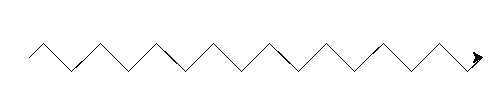
\includegraphics[width=0.5\textwidth]{img/pattern.png}
    \caption{Rectangle pattern.}
    \label{fig:enter-label}
\end{figure}

Next, experiment a bit and implement your own ideas. Following is another example of a pattern created from circles. Be creative!

\begin{figure}[!h]
    \centering
    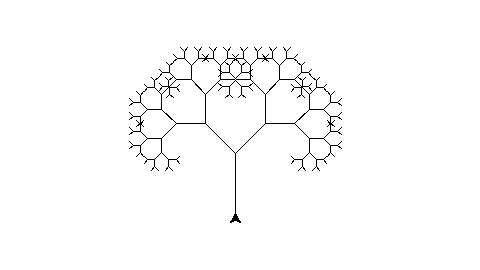
\includegraphics[width=0.5\textwidth]{img/pattern2.png}
    \caption{Circle pattern.}
    \label{fig:enter-label}
\end{figure}

\end{task}

\newpage


\begin{task}{Recursive spiral}{}{}

Implement a recursive function \code{spiral(int: size, float: angle, float: scale, int: maxSize)} that draws spirals like the example below.

\begin{figure}[!h]
    \centering
    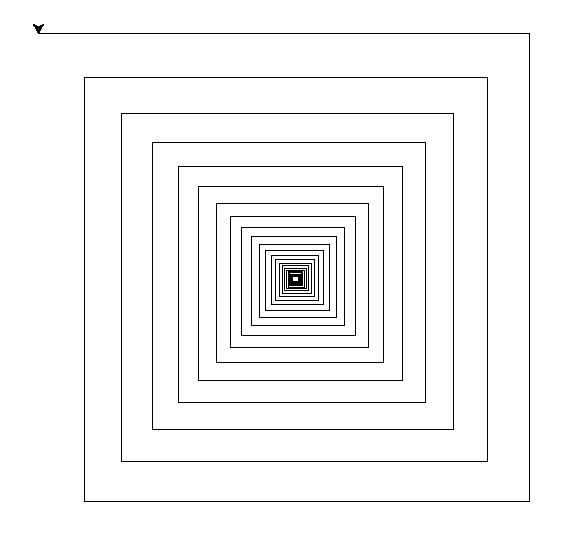
\includegraphics[width=1\textwidth]{img/spiral.png}
    \caption{A spiral.}
    \label{fig:enter-label}
\end{figure}

\end{task}

\newpage

\begin{task}{Recursive tree}{}{}

Implement a recursive function \code{tree(int: branches, int: size, float: angle, float: scale)} that draws trees like the examples below. 

\begin{figure}[!h]
    \centering
    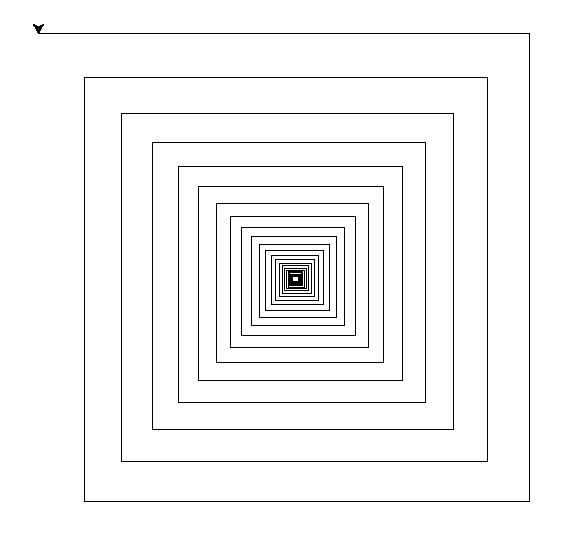
\includegraphics[width=1\textwidth]{img/tree45.png}
    \caption{A tree created with $45^{\circ}$ angles.}
    \label{fig:enter-label}
\end{figure}

\begin{figure}[!h]
    \centering
    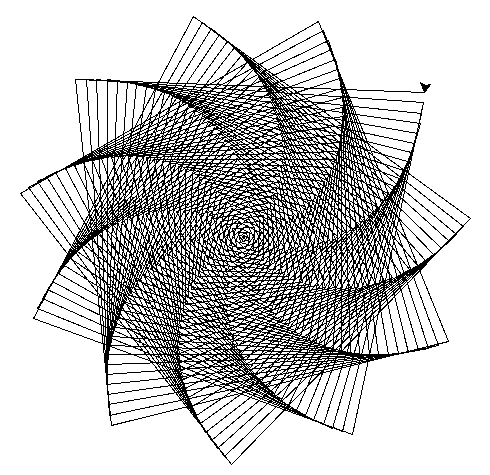
\includegraphics[width=1\textwidth]{img/tree90.png}
    \caption{A tree created with $90^{\circ}$ angles.}
    \label{fig:enter-label}
\end{figure}

\end{task}

\clearpage
\section{Douglas Peucker Algorithm, Recursion}

\begin{task}{The Douglas-Peucker Algorithm}{}{}
The Douglas-Peucker algorithm (also Ramer-Douglas-Peucker algorithm) is an algorithm that decimates a curve composed of line segments to a similar curve with fewer points.
It was one of the first efficient algorithms for cartographic generalization.
First, find a suitable source and familiarize yourself with the algorithm.
\end{task}


\begin{task}{Implement the Douglas-Peucker Algorithm}{}{}
Implement the Douglas-Peucker algorithm to simplify trajectories.
Test it on a simple artificial trajectory and visualize the original and simplified trajectory with \code{matplotlib}. For example, your trajectory for testing may look like this:
\begin{lstlisting}[numbers=none]
T = [[1,1],[2,3],[3,4],[5,1],[6,2],[8,3],[10,5]]
\end{lstlisting}

\vspace{10pt}

\textbf{Additional Information:}
\begin{itemize}
    \item As input, the Douglas-Peuker algorithm is given a trajectory as a sequence of points (timestamps are not needed) and an error threshold epsilon. 
    \item It starts by trying to approximate the trajectory with the shortest trajectory possible, containing only the start and end points. 
    \item It proceeds from such shortest trajectories by finding the point of largest error and adding the point of the original trajectory into the current simplification until this error is smaller than epsilon.
    \item The resulting trajectory is the simplification.
\end{itemize}


\textbf{Implementation Hints:}
\begin{itemize}
    \item You need to implement a point line distance function.
    \item You can implement the simplification using a property map approach: An array of boolean values of the same size as the trajectory can be updated if a point needs to be inserted.
    \item It makes sense to have a findMaxError function returning the size of the error and the location.
    \item As a variation, you can replace the epsilon with a point budget like "simplify as long as the number of points is smaller than my budget".
\end{itemize}

\end{task}


\begin{task}{Apply the Douglas-Peucker Algorithm}{}{}
Apply the algorithm to a large polygon and test different values for epsilon. 
It is suggested to take, for example, the administrative border of a country of your choice (you can download shapefiles for most countries \href{https://www.diva-gis.org/gdata}{here}), but you may also use any other large polygon.
You can read shapefiles with the \href{https://pypi.org/project/pyshp/}{PyShp} package.
Below is a way to read in a shapefile with PyShp.

\begin{lstlisting}
import shapefile as shp 

sf = shp.Reader(file)

x = []
y = []
for shape in sf.shapeRecords():
    x.append([i[0] for i in shape.shape.points[:]])
    y.append([i[1] for i in shape.shape.points[:]])
\end{lstlisting}

Finally, think about ways to optimize your code.

\end{task}


\clearpage
\section{Solving complex computational problems Pt1}

In this longer tutorial, we want to jointly look at how we can combine our initial knowledge to build a full deep learning system in which a large spatial image and GDAL are used together with Tensorflow to predict a certain spatial feature.

\vspace{10pt}

In this first part, we will build knowledge on GDAL, cut out small images (called tiles or patches) from your measured data, and assign a class to it.

%In the beginning, it is proposed to build knowledge on the three involved aspects individually:
%- understand the GDAL workbook and already try to extract smaller patches (therefore, check the example GDAL notebook!)
%- learn about the simple deep learning example (keras, mnist) which can detect handwritten letters in black and white. Maybe extend it to RGB images already (you could build an RGB image from three identical grayscale layers)


\begin{task}{Data exploration}{}{}
Initially, it is proposed to build knowledge on GDAL and understand the provided data \code{germany.tiff}.
Therefore, go through the script \code{GDAL.ipynb}, then try to adapt it.
Choose a point of interest (POI) and extract the area around it as a JPG file for further processing.
Finally, you should end up with an RGB image file \code{germany\_poi.jpg}.

\end{task}

\begin{task}{Create tiles}{}{}
Tile the file \code{germany\_poi.jpg} from Task 1 by writing a function \code{tile()}.
It is suggested to create tiles/patches with a size of $48 \times 48$ or $64 \times 64$, but you may choose any size you like.
Also, try to overlap the tiles by a small amount.
Finally, save the tiles in a new directory.

\end{task}

\begin{task}{Ground truth}{}{}
Before we can run a deep learning model, we need ground truth data.
You may use any ground truth for any spatial feature you like.
However, here, we will use, as an example, forest as a spatial feature and download it via the Overpass API.
Overpass-turbo is a web-based data mining tool for Open Street Map and can be accessed \href{https://overpass-turbo.eu/}{here}.
You can read the documentation on the API and how to write queries \href{https://wiki.openstreetmap.org/wiki/Overpass_API/Overpass_QL}{here}.
Then, we import the extracted geojson file with QGIS or ArcGIS, rasterize the data, and export it as TIFF (in QGIS click "Raster", "Conversion", then "Rasterize").
It is important to extract the TIFF with the right coordinate system and bounding box applied.

\end{task}


\begin{task}{Label the data}{}{}
Finally, write a function \code{label\_data()} to assign a class to the tiles.
Here, the simplest approach is to extract a random patch (random location, but within the bounds of the image), and if it contains forest (\code{np.sum(...) != 0}), you store a JPG file of the patch in a directory \code{no\_forest}. Otherwise, put it into \code{forest}.
You end up with two directories of images.

\end{task}

\clearpage
\section{Solving complex computational problems Pt2}
In this second part, we will learn about Keras data loaders and train a neural network to detect some spatial features.
It is proposed that knowledge on Keras be first built with a tutorial for a simple deep-learning example. 
A beginner-friendly overview can be found \href{https://www.tensorflow.org/tutorials/keras/classification}{here}.
Note that for multidimensional raster data, you may want to use convolutional layers like shown \href{https://keras.io/examples/vision/mnist_convnet/}{here}.
You may even extend the example with RGB images already (you could build an RGB image from three identical grayscale layers).


\begin{task}{Data loading}{}{}
A convenient way to load and prepare your data for deep learning with Keras is a "data loader".
You can read the official documentation and examples \href{https://keras.io/api/data_loading/}{here} and subsequently \href{https://keras.io/api/data_loading/image/}{here}.
Set up data loaders for train, test, and validation data.
\end{task}

\begin{task}{Deep learning model}{}{}
Build and compile a deep learning model with Keras.
You may adapt the convolutional neural network from \href{https://keras.io/examples/vision/mnist_convnet/}{this} example.
\end{task}

\begin{task}{Training and evaluation}{}{}
Finally, train (\code{model.fit()}) and evaluate (\code{model.evaluate()}) your model.
Plot some examples for correct and wrong classified images.
\end{task}


\begin{task}{Improvements}{}{}
Think about ways to improve your model.
You may, for example, try to use data augmentation (which is quite easy with Keras data loaders) or enlarge your training area (and thus the number of training samples).
Further, you may increase or decrease the learning rate and the number of training epochs.

\end{task}

\clearpage
\section{Become a practitioner with Data Mining tasks.}

\begin{task}{Mining Approaches}{}{}

Starting from the \textit{LiveCoding} notebook and dataset (\url{https://www.moodle.tum.de/course/section.php?id=3718743} apply different supervised and unsupervised techniques to create a model.

\begin{itemize}
    \item Clustering
    \item Regression
    \item Classification
    \item Decision Tree
    \item ...
\end{itemize}
\vspace{10pt}


You can use other data and approaches from the lecture (see data mining notebooks).


\end{task}

\begin{task}{Model Evaluation}{}{}

The evaluation of your models is a crucial step. Calculate and interpret evaluation metrics for your models (following \url{https://www.moodle.tum.de/mod/resource/view.php?id=3246274}).


\end{task}

\begin{task}{SQL*}{}{}

Manage your patches in SQLite and make them accessible via API with `fire` (\url{https://github.com/google/python-fire}).


\end{task}

\newpage
\section{Multilateration}
"Pseudo-range multilateration, often simply multilateration when in context, is a technique for determining the position of an unknown point, such as a vehicle, based on measurement of the times of arrival of energy waves traveling between the unknown point and multiple stations at known locations." [\href{https://en.wikipedia.org/wiki/Pseudo-range\_multilateration}{Wikipedia}]

\begin{task}{Multilateration}{}{}

Write a program to perform multilateration.
You should first review the lecture slides and familiarize yourself with the algorithm.
\vspace{10pt}

\noindent Following is a summary of the algorithm:
\begin{enumerate}
    \item Set up a non-linear system of equations from measurements.
    \item Create a linearized version locally by choosing an initial value and using Taylor expansion at this point.
    \item Solve this equation and obtain an update vector.
    \item Update this and go back to b. with this new place information
\end{enumerate}
\vspace{5pt}
Thus, implement the following steps:
\begin{enumerate}
    \item Calculate distances:
$\alpha_{i}=\sqrt{(x_{i}-\Tilde{x})^2+(y_{i}-\Tilde{y})^2}$ for $i = 1, ..., 4$.
    \item Build matrix:
$A_{i}=(-\frac{(x_{i}-\Tilde{x})}{\alpha_{i}}, -\frac{(y_{i}-\Tilde{y})}{\alpha_{i}})$.
    \item Create: $b_{i}=d_{i}-\alpha_{i}$.
    \item Solve: $A\begin{pmatrix}\hat{x}\\\hat{y}\end{pmatrix}=b$.
    \item Compute: $\begin{pmatrix}\Tilde{x}_{2}\\\Tilde{y}_{2}\end{pmatrix}= \begin{pmatrix}\Tilde{x}_{1}\\\Tilde{y}_{1}\end{pmatrix} + \begin{pmatrix}\hat{x}\\\hat{y}\end{pmatrix}$.
\end{enumerate}

\clearpage
You can use the following data from the lecture:\\
\\
\begin{tabularx}{0.8\textwidth} { 
  | >{\raggedright\arraybackslash}X 
  | >{\raggedright\arraybackslash}X 
  | >{\raggedright\arraybackslash}X | }
 \hline
 \textbf{Component} & \textbf{Coordinate} & \textbf{Measurement} ($d_{j}$) \\
 \hline
 Base station 1  & $(x_{1}, y_{1}) = (0, 0)$  & $2.92$ \\
 \hline
 Base station 2  & $(x_{2}, y_{2}) = (10, 0)$  & $8.14$ \\
 \hline
 Base station 3  & $(x_{3}, y_{3}) = (15, 10)$  & $15.46$ \\
 \hline
 Base station 4  & $(x_{4}, y_{4}) = (0, 12)$  & $9.89$ \\
 \hline
 Mobile Device  & $(x_{e}, y_{e}) = (2, 2)$  & $-$ \\
 \hline
 Initial Location Estimate  & $(\Tilde{x}, \Tilde{y}) = (20, 20)$  & $-$ \\
\hline
\end{tabularx}

\end{task}


\newpage
\section{Exam Preparation}

In this tutorial, we practice a mock exam.

\vspace{10pt}

\begin{task}{State your Name}{}{}

Name: \\
 \\
 \\
Surname: \\
 \\
 \\

\end{task}

\begin{task}{Yes-No-Example}{}{}
Answer the following questions with yes or no. \\

\begin{yesnolist}
  \yesnoquestion{In Python, you need to define a function to execute a script.}{X}{}{}
  \yesnoquestion{The Numpy and Matplotlib library are by default part of the Python installation.}{X}{}{}
  \yesnoquestion{To install a Python package, you always have to create a virtual environment.}{X}{}{} 
\end{yesnolist}
\end{task}

\clearpage

\begin{task}{Multiple Joice Example}{}{}
For the given question, one of the answer options is correct. Mark this (and only this) answer. If more than one answer is marked, the answer is not considered. A wrong answer is \textbf{not} counted as -1.\vspace{1cm}

  \begin{multiplechoice}{In programming, what is meant by a recursive function?}
    \mcanswer{A function that is called multiple times.}{}
    \mcanswer{A function that calls itself.}{}
    \mcanswer{A function inside another function.}{}
    \mcanswer{A function that takes another function as input.}{}
  \end{multiplechoice}

  \begin{multiplechoice}{Which of the following is \textbf{not} a method of a list object in Python?}
    \mcanswer{remove}{X}
    \mcanswer{delete}{}
    \mcanswer{reverse}{}
    \mcanswer{pop}{}
  \end{multiplechoice}
\end{task}


\begin{task}{Distance Between Two Points}{}{}
Complete the given Python function \code{dist()} that takes two points \code{p1 = [x1, y1]} and \code{p2 = [x2, y2]} as input and shall return their distance.
\begin{lstlisting}
    def dist(p1, p2):
        # ...
        return distance
\end{lstlisting}
\end{task}

\clearpage

\begin{task}{List Comprehension}{}{}
  \begin{enumerate}
  \item{Consider the following program using list expressions.}
  \begin{lstlisting}
  vocabulary = ['dear', 'done', 'easy', 'hello', 'hope', 'is', 'it', 'say', 'student', 'to', 'we', 'well']
  sentence = " ".join([vocabulary[x] for x in [3,0,8,10,4,6,5,2]])
  print(sentence)
  \end{lstlisting}
  Give the exact output of the program 

\vspace*{6cm}


  \item{Consider the following Python function consisting of seven lines of code.}
  \begin{lstlisting}
  def myFunction(n: list):
      result = []
      for k in n:
          if k > 0:
              tmp = k**2
              result.append(tmp)
      return result
  \end{lstlisting}
  Rewrite the function with a list comprehension such that it only needs two lines of code.
  \end{enumerate}

\end{task}

\end{document}